\documentclass[main.tex]{subfiles}
\usepackage[utf8]{inputenc}
\usepackage[
backend=biber,
style=alphabetic,
sorting=ynt
]{biblatex}


\addbibresource{references.bib} %Imports bibliography file

% Document information
\title{Estado del arte}
\author{Rocío Mena}
\date{\today}

\begin{document}

\maketitle

\section{Políticas orientadas a la sustentabilidad}

La transición hacia prácticas más sostenibles y respetuosas con el medio ambiente es uno de los desafíos más significativos y urgentes que enfrentan las sociedades contemporáneas. En este contexto, las políticas públicas orientadas a la sustentabilidad ecológica desempeñan un papel crucial en la modelación de estrategias que no solo buscan mitigar los efectos del cambio climático, sino también transformar la economía global hacia modelos más circulares y regenerativos. Estas políticas están diseñadas para integrar tres dimensiones del desarrollo sostenible: la económica, la social y la ambiental, ofreciendo así una hoja de ruta integral que articula la acción colectiva en torno a objetivos comunes que son tanto ambientales como socioeconómicos \cite{gil2018objetivos}.

En el ámbito de América Latina, por ejemplo, se han implementado modelos de economía circular que intentan reformular el uso y gestión de los recursos, promoviendo la reducción, reutilización y reciclaje de materiales \cite{rodriguez2023modelamiento, cepal2021economia}. Estas iniciativas son fundamentales para enfrentar los retos locales y globales de la gestión de residuos y la preservación de recursos naturales. En este sentido, la Estrategia Nacional de Consumo y Producción Sostenibles de Argentina representa un esfuerzo significativo por parte del gobierno para alinear las prácticas de consumo y producción con los Objetivos de Desarrollo Sostenible (ODS) de las Naciones Unidas, enfocándose específicamente en el ODS 12, que promueve un consumo y producción responsables \cite{sostenible2021argentina}.

Sin embargo, a pesar de los avances en la formulación de políticas, la implementación efectiva enfrenta desafíos significativos. La complejidad de las estructuras económicas existentes, la falta de compromiso a largo plazo y las necesidades de inversiones considerables para tecnologías sostenibles son solo algunas de las barreras que estos países deben superar. Además, la eficacia de estas políticas frecuentemente se ve limitada por la falta de coherencia y coordinación entre diferentes niveles de gobierno y sectores de la sociedad, así como por la insuficiencia de indicadores claros y medibles para evaluar el progreso hacia los objetivos propuestos \cite{gil2018objetivos}.

A pesar de los esfuerzos legislativos y las iniciativas implementadas, es evidente que el impacto real de las políticas públicas orientadas a la sustentabilidad ecológica, aunque positivo en cierta medida, no ha alcanzado el nivel de efectividad esperado \cite{gil2018objetivos, clima2022book}. De manera generalizada, el impacto positivo de estas políticas ha sido insuficiente para contrarrestar de manera significativa el impacto ambiental negativo de las sociedades en las que se han implementado, dentro del período acordado. Esto resalta una brecha crítica entre los objetivos propuestos y los resultados tangibles obtenidos, subrayando la necesidad urgente de reevaluar y fortalecer los mecanismos de acción y cumplimiento. La insuficiencia de estas políticas para neutralizar los efectos adversos en el tiempo establecido indica un desafío persistente en la política de desarrollo sostenible global.

En conclusión, mientras que la formulación de políticas públicas orientadas a la sustentabilidad ecológica es un paso vital hacia un desarrollo más sostenible, la clave para su éxito radica en la capacidad de implementar estos marcos de manera efectiva, garantizando que las transiciones hacia modelos circulares y sostenibles sean viables, inclusivas y beneficiosas para cada actor del modelo. A continuación se exploran una serie de políticas específicas implementadas en diversos contextos, evaluando su impacto, efectividad y las lecciones aprendidas en el proceso.

\subsection{Evolución de las Políticas de Cambio Climático y la Neutralidad Climática en la Unión Europea}

En el marco del Pacto Verde Europeo, la Unión Europea ha otorgado rango legal a su objetivo de neutralidad climática mediante la Ley Europea del Clima, impulsando una serie de políticas innovadoras para su implementación, como el paquete de medidas conocido como Objetivo 55 \cite{dormido2022cambio}.

\subsubsection{De Río a París: Hitos en la Acción Climática}
La trayectoria internacional de la acción frente al cambio climático ha evolucionado significativamente desde los acuerdos iniciales en Río de Janeiro en 1992. Este cambio refleja una mayor comprensión de la influencia humana sobre el clima y sus implicaciones económicas, culminando en la adopción de la Convención Marco de las Naciones Unidas sobre el Cambio Climático (CMNUCC). Los esfuerzos continuaron con el Protocolo de Kyoto en 1997, que estableció por primera vez compromisos de reducción de emisiones de CO2 para los países desarrollados \cite{dormido2022cambio}.

\subsubsection{El Acuerdo de París y su Implementación}
El Acuerdo de París, firmado en 2015, marca un hito histórico al ser el primer tratado internacional universal sobre el cambio climático. Este acuerdo compromete a sus signatarios a mantener el aumento de la temperatura global por debajo de los 2ºC con respecto a los niveles preindustriales y esforzarse por limitar este aumento a 1,5ºC. Además, se establecen mecanismos para la mitigación, adaptación y resiliencia ante el cambio climático, incluyendo un marco financiero y técnico para apoyar a los países más vulnerables \cite{dormido2022cambio}.

\subsubsection{Acciones del G-20 y la Economía Circular}
En respuesta a la crisis del COVID-19, los asuntos climáticos han ganado protagonismo en la agenda del G-20, reflejando la urgencia de estas políticas. Los comunicados del G-20 han resaltado la importancia de asignar recursos financieros adecuados para la mitigación del cambio climático y la adopción de tecnologías limpias para alcanzar emisiones cero, así como el acceso a fuentes de energía limpia. Además, se destaca el acuerdo para la reducción de emisiones de metano, consideradas clave en la estrategia de mitigación rápida y económica del cambio climático \cite{dormido2022cambio}.

\subsubsection{Impuestos al Carbono y Políticas Fiscales Sostenibles}
Las recomendaciones del Fondo Monetario Internacional enfatizan la necesidad de un impuesto global al carbono como la medida más eficiente para la descarbonización. A nivel nacional, se sugieren reformas en los subsidios a los combustibles fósiles y el fomento de inversiones en energías verdes, complementadas con transferencias para compensar a los hogares vulnerables por los efectos de la transición energética \cite{dormido2022cambio}.

\subsubsection{El Pacto Verde Europeo}
Adoptado en 2019, el Pacto Verde Europeo es el compromiso programático más reciente de la UE en la lucha contra el cambio climático. Este pacto busca transformar los retos climáticos y ambientales en oportunidades para todas las áreas de actuación, promoviendo una transición justa e integradora hacia una economía sostenible y climáticamente neutra para 2050. El principal desafío de implementar el Pacto Verde y otras políticas similares radica en la necesidad de una transición justa que compense a las comunidades afectadas por los cambios industriales \cite{dormido2022cambio}.

\subsubsection{Iniciativa Close the Glass Loop}
La iniciativa Close the Glass Loop es un esfuerzo colaborativo para alcanzar una tasa de recolección empaques de vidrio para reciclaje del 90\% en la UE para 2030. Este programa no solo promueve la recolección de vidrio, sino que también fomenta el uso del vidrio reciclado en la producción de nuevos envases, cerrando así el ciclo de vida del material. A través de una serie de asociaciones estratégicas y campañas de comunicación intensivas, Close the Glass Loop trabaja para aumentar la conciencia y mejorar las infraestructuras de reciclaje, con el objetivo de transformar la gestión de residuos de vidrio y lograr un cambio sistemático en toda la industria \cite{closetheglassloop2023}. Hasta el año 2024, esta iniciativa ya ha alcanzado una tasa de recolección y reciclaje mayor al 80\% en la UE, lo que representa un avance significativo hacia el objetivo final \cite{closetheglassloop2023}.

\subsection{Objetivos de Desarrollo Sostenible}
Los Objetivos de Desarrollo Sostenible (ODS), establecidos por la Organización de las Naciones Unidas (ONU) en 2015 como parte de la Agenda 2030 para el Desarrollo Sostenible, son un marco global compuesto por 17 objetivos interconectados. Estos objetivos representan un esfuerzo global para erradicar la pobreza, proteger el medio ambiente, y garantizar que todas las personas disfruten de paz y prosperidad para 2030. Son el consenso más amplio a lo que la humanidad aspira en cuanto a un futuro deseable y abordan las dimensiones económica, social y ambiental del desarrollo sostenible a través de metas concretas y cuantificables. Los objetivos se materializan en 169 metas concretas medibles a través de 230 indicadores, diseñados para ser aplicados universalmente a todos los países  \cite{onu2024ods gil2018objetivos}.

Varios ODS están directamente relacionados con la economía circular y la sostenibilidad ecológica, destacando la importancia de:

\begin{itemize}
		\item \textbf{ODS 7: Energía asequible y no contaminante.} Garantiza el acceso universal a servicios energéticos asequibles, confiables, sostenibles y modernos.
    \item \textbf{ODS 11: Ciudades y comunidades sostenibles.} Se enfoca en hacer que las ciudades y los asentamientos humanos sean inclusivos, seguros, resilientes y sostenibles.
    \item \textbf{ODS 12: Producción y Consumo Responsables} — Fomenta prácticas sostenibles que incluyen la reducción del desperdicio mediante la prevención, reciclaje y reutilización.
    \item \textbf{ODS 13: Acción por el Clima} — Insta a la adopción de medidas urgentes para combatir el cambio climático y sus efectos.
    \item \textbf{ODS 14 y 15: Vida Submarina y Terrestre} — Promueven la conservación y uso sostenible de los ecosistemas oceánicos y terrestres, esenciales para la biodiversidad y la sostenibilidad ambiental.
\end{itemize}

Los ODS ofrecen una visión integradora y global del desarrollo sostenible. Sin embargo, para que esta visión se materialice en acciones efectivas y resultados tangibles, se requiere un compromiso profundo y coordinado a nivel internacional, junto con estrategias adaptadas a las realidades locales de cada país \cite{gil2018objetivos}.
Los ODS, como un marco global para el desarrollo sostenible, necesitan acciones concertadas y compromisos políticos claros para ser efectivos. La comunidad internacional debe priorizar estos objetivos dentro de sus políticas nacionales y cooperar a nivel internacional para asegurar que los esfuerzos sean inclusivos y efectivos en todos los sectores de la sociedad \cite{onu2024ods}.

A pesar de la amplitud y la ambición de los ODS, han surgido críticas significativas respecto a su estructura y efectividad. La complejidad de su arquitectura y las limitaciones técnicas han sido puntos de preocupación, así como la falta de compromisos específicos y medibles que aseguren su cumplimiento. Los ODS han sido criticados por ser en gran parte retóricos y ambiciosos sin suficientes directrices claras para su implementación, lo que ha generado disparidades en la aplicación entre diferentes países \cite{gil2018objetivos}.

Los ODS requieren un cambio significativo en las políticas y prácticas globales, lo cual ha sido un proceso complejo y desigual entre los países. Los estados han encontrado dificultades para avanzar en la implementación de estas metas, debido en parte a la falta de indicaciones claras sobre cómo llevar a cabo estas transformaciones. Además, la voluntariedad de los ODS permite que cada país avance a su propio ritmo, lo que podría resultar en esfuerzos dispersos y no coordinados \cite{gil2018objetivos}.

A pesar de la ambición de los ODS sobre el progreso ecológico y la sostenibilidad global, el impacto real hasta la fecha ha sido mixto en comparación con las proyecciones iniciales. Según el análisis presentado en \textit{Clima} \cite{clima2022book}, la implementación de los ODS ha enfrentado desafíos significativos, incluyendo la falta de recursos financieros, políticas incoherentes a nivel nacional, y la necesidad de mayor cooperación internacional. Aunque se han hecho avances en algunos sectores, el progreso global hacia metas críticas como la reducción de emisiones de gases de efecto invernadero y la conservación de la biodiversidad ha sido insuficiente para cumplir con los objetivos establecidos para 2030. Este desfase subraya la necesidad urgente de revisar las estrategias y compromisos, tanto a niveles nacionales como internacionales, para asegurar que los avances hacia la sostenibilidad ecológica no solo sean aspiracionales sino efectivos y tangibles.

\subsubsection{Estrategias de Desarrollo Productivo Verde}
El capítulo sobre políticas de desarrollo del FUNDAR subraya la importancia de integrar dimensiones económicas, sociales y ambientales en el desarrollo. Busca avanzar hacia una estructura productiva que maximice la eficiencia en el uso de recursos y minimice el impacto ambiental. 

Las políticas sostenibles enfrentan limitaciones significativas debido a la complejidad de los sistemas económicos y la falta de un marco regulatorio coherente. La implementación efectiva de estas políticas se ve obstaculizada por estos factores, junto con la resistencia de sectores arraigados y la insuficiencia de inversiones en tecnologías limpias.

\subsection{Políticas Sustentables y Gestión de Residuos en América Latina}

\subsubsection{Introducción a la Economía Circular y su Impacto Macroeconómico}
La transición hacia una economía circular en América Latina no solo implica un cambio en la gestión de residuos sino que también ofrece una oportunidad para mejorar la macroeconomía de la región. En el estudio \textit{Modelamiento de los efectos macroeconómicos de la transición a la economía circular en América Latina} \cite{rodriguez2023modelamiento}, se exploran los impactos potenciales en el empleo, la huella climática, y el Producto Interno Bruto (PIB) mediante un modelo que simula diferentes escenarios de transición. Este modelo destacó que, con una reducción conservadora en el uso de materiales como el plástico y el cemento, los países podrían ver incrementos en el PIB de hasta 2.2\% y mejoras en el empleo de hasta 2.1\% para 2030, además de reducciones en las emisiones de gases de efecto invernadero (GEI), mostrando un potencial para recuperaciones verdes \cite{rodriguez2023modelamiento}.

\subsection{Políticas Públicas y Avances en la Gestión de Residuos}
Según el documento \textit{Economía Circular en América Latina y el Caribe: oportunidad para una recuperación transformadora} \cite{cepal2021economia}, la región ha implementado diversas políticas para fomentar la economía circular, que incluyen legislaciones sobre la responsabilidad extendida del productor y prohibiciones de plásticos de un solo uso. Estas políticas buscan no solo reducir la generación de residuos sino también promover la reutilización y el reciclado, integrando aspectos económicos, sociales y ambientales en línea con la Agenda 2030 para el Desarrollo Sostenible \cite{cepal2021economia}.

A pesar de los avances, existen desafíos significativos debido al déficit en infraestructura para la gestión de residuos y las bajas tasas de reciclaje, que están muy centradas en pocos productos, como el papel y el cartón. Estas limitaciones ofrecen, sin embargo, una ventana de oportunidad para mejorar la gestión de residuos y promover la economía circular a nivel local, utilizando cadenas productivas que potencien el desarrollo sostenible \cite{cepal2021economia}.

\subsubsection{Estrategias Legislativas y Normativas}
La implementación de leyes de responsabilidad extendida del productor en la región ha sido un paso importante para asegurar que los fabricantes asuman una parte del costo y la gestión de sus productos al final de su vida útil. Sin embargo, el impacto de estas políticas aún está limitado por la falta de un sistema integral que involucre a todos los actores, desde consumidores hasta gestores de residuos y el Estado, para garantizar una gestión eficiente de los residuos \cite{cepal2021economia}.

Según Rodríguez \cite{rodriguez2023modelamiento}, es crucial usar la experiencia adquirida en la modelación inicial para desarrollar modelos más complejos que integren los efectos ambientales. Esto incluye la adaptación del modelo a diferentes contextos macroeconómicos y sectores, lo que permitirá una aplicación más amplia de la economía circular en América Latina. Además, es esencial fortalecer la construcción de indicadores y metas físicas para una transición efectiva hacia la economía circular.

Ambos informes conciden en que la transición hacia la economía circular en América Latina presenta una oportunidad única para alinear los objetivos económicos con los ambientales y sociales, promoviendo un desarrollo sostenible y resiliente. Sin embargo, se requiere una colaboración más estrecha entre los gobiernos, la industria y la sociedad civil para superar los desafíos actuales y maximizar los beneficios de las políticas implementadas. La continuidad en la evaluación y ajuste de las políticas será crucial para garantizar que la región pueda alcanzar los objetivos establecidos para 2030 y más allá \cite{cepal2021economia}.

\subsection{Políticas Sustentables en Argentina}
En Argentina, las políticas de desarrollo sostenible han cobrado una importancia significativa en respuesta a la crisis climática global y a la necesidad de promover un desarrollo económico que sea ambiental y socialmente responsable. Los esfuerzos del país para implementar estas políticas están alineados con los ODS y reflejan un compromiso con la transformación hacia prácticas de producción y consumo sostenibles \cite{dormido2021fundar, sostenible2021argentina}.

\subsection{Desarrollo Productivo Verde}

Según FUNDAR, un laboratorio de políticas públicas argentino, es crucial que el Estado, el mercado y la sociedad civil trabajen conjuntamente para enfrentar los retos ambientales. Este enfoque colaborativo es esencial para diseñar políticas que no solo apunten a reducir las emisiones de gases de efecto invernadero sino que también fomenten la independencia y el crecimiento económico sostenible de Argentina \cite{dormido2021fundar}.

\subsection{Estrategia Nacional de Consumo y Producción Sostenibles}

La "Estrategia Nacional de Consumo y Producción Sostenibles" representa un esfuerzo significativo por parte del gobierno argentino para integrar la sostenibilidad en todos los aspectos de la cadena de producción y consumo. La estrategia incluye medidas en educación, regulaciones políticas, promoción de tecnologías sostenibles, gestión de recursos y sostenibilidad en la cadena de valor \cite{sostenible2021argentina}.

\subsubsection{Componentes Clave de la Estrategia}

\begin{itemize}
    \item \textbf{Educación y Sensibilización:} Incrementar la conciencia sobre la importancia de prácticas sostenibles.
    \item \textbf{Políticas Regulatorias:} Implementar leyes que incentiven el uso de prácticas y tecnologías sostenibles en la industria.
    \item \textbf{Promoción de Tecnologías Sostenibles:} Apoyar el desarrollo y adopción de tecnologías que minimicen el impacto ambiental.
    \item \textbf{Gestión Sostenible de Recursos:} Fomentar el uso eficiente de recursos y la reducción de residuos.
    \item \textbf{Integración de la Sostenibilidad en la Cadena de Valor:} Aplicar criterios de sostenibilidad en compras públicas y privadas.
\end{itemize}

La estrategia ha tenido impactos multidimensionales, destacando mejoras en la competitividad económica, conservación de ecosistemas y empoderamiento social. Sin embargo, los desafíos incluyen la necesidad de mayor participación del sector privado y la efectiva implementación de políticas a nivel local y regional \cite{sostenible2021argentina}.

La evaluación del impacto real sobre las emisiones de GEI y la efectividad general de las políticas sostenibles en Argentina es un tema de debate. A pesar de los avances, la implementación efectiva de estas políticas enfrenta desafíos significativos, incluyendo la falta de recursos financieros, la resistencia de sectores arraigados y la necesidad de inversiones en tecnologías limpias. La colaboración entre el gobierno, la industria y la sociedad civil será fundamental para alcanzar los objetivos ambientales y de desarrollo sostenible del país \cite{dormido2021fundar, sostenible2021argentina}.


\section{Programas de Reciclaje de Vidrio en Argentina}

En Argentina, diversos programas han sido implementados para fomentar el reciclaje de vidrio, destacando las cualidades sostenibles y reciclables de este material. Estos programas varían en enfoque y escala, pero todos comparten el objetivo común de maximizar el reciclaje de vidrio. Mientras que el vidrio es un material altamente reciclable, en caso de no ser reciclado, puede tardar miles de años en descomponerse en un vertedero, lo que lo convierte en un material altamente contaminante \cite{cordoba2024vidrio}. Su tasa de reciclaje en Argentina es relativamente baja en comparación con otros países, lo que ha motivado la implementación de estos programas para promover su reciclaje y reutilización \cite{vidriotransparente2024mendoza, innovar2024vidrio, cordoba2024vidrio}.

\subsection{Verallia - Vidrio una Iniciativa Solidaria}
Este programa, mencionado anteriormente, es un esfuerzo conjunto entre Verallia y el Gobierno de Mendoza, conocido como "Vidrio, una acción transparente" \cite{vidriotransparente2024mendoza}. Promueve activamente la recolección y reciclaje de vidrio, beneficiando no solo el medio ambiente sino también la economía local y el bienestar social mediante el apoyo a organizaciones benéficas con los ingresos generados del vidrio reciclado. 

\subsection{San Isidro + Reciqlo}
El Municipio de San Isidro, en colaboración con la organización Reciqlo, lanzó un innovador programa de reciclado de vidrio a domicilio, el primero de su tipo en el país. Este programa facilita la recolección de vidrio utilizando un camión especial que visita las casas semanalmente. Los vecinos inscritos en el programa depositan sus envases de vidrio en un cajón proporcionado por Reciqlo, que luego son recogidos y transportados a la planta de reciclaje. El vidrio reciclado se utiliza posteriormente en proyectos de impacto urbano como el bacheo en frío y la mejora de suelos para espacios verdes \cite{innovar2024vidrio}.

\subsection{Vidrio Sí, Gracias - Córdoba}
El proyecto "Vidrio sí, gracias" en Córdoba es otro ejemplo de iniciativa local que fomenta la participación comunitaria en el reciclaje de vidrio. Este programa no solo ayuda a reducir la cantidad de vidrio que llega a los basurales sino que también involucra a los recuperadores locales en el proceso, garantizando que formen parte activa del proyecto de reciclaje \cite{cordoba2024vidrio}.

\subsection{Conclusión}

Estos programas reflejan un compromiso sustancial con la sostenibilidad y la economía circular, destacando el papel significativo de los municipios o gobiernos locales en la promoción del reciclaje. Sin embargo, aún existen desafíos en términos de concientización, participación y logística que deben abordarse para maximizar el impacto de estas iniciativas. 

En la revisión de los programas de reciclaje de vidrio en Argentina, no se han encontrado métricas específicas que indiquen la tasa de adopción o la cantidad exacta de material efectivamente reciclado. Estos programas están diseñados para simplificar la logística del reciclaje para el usuario final, promoviendo la facilidad de entrega y procesamiento del vidrio. Sin embargo, estos sistemas no garantizan por sí mismos el reciclaje efectivo de los residuos, ni ofrecen incentivos o imposiciones que obliguen a los ciudadanos a participar. En cambio, dependen principalmente de la buena voluntad de los individuos para su éxito. A diferencia de estas iniciativas, programas como Close the Glass Loop en Europa \cite{closetheglassloop2020ue} han demostrado que la implementación de incentivos claros y estrategias más estructuradas puede significativamente aumentar las tasas de reciclaje, sugiriendo que una aproximación más robusta podría ser necesaria para lograr resultados similares en Argentina.

\section{Aplicaciones con incentivos al reciclaje}
Esta sección explora aplicaciones productivas que utilizan incentivos para fomentar mejores resultados en reciclaje. Estas aplicaciones parten de la idea de que la motivación económica puede ser un factor clave para aumentar la participación ciudadana en el reciclaje. Al ofrecer recompensas tangibles a los usuarios por sus acciones sostenibles, estas aplicaciones buscan cambiar el comportamiento y fomentar hábitos más responsables con el medio ambiente en sus usuarios.

\subsection{Reciclos}
\textbf{Reciclos} es una aplicación de reciclaje con base en España que funciona como un Sistema de Devolución y Recompensa (SDR). Los usuarios ganan puntos por reciclar latas y botellas de bebida, que luego pueden cambiar por incentivos sostenibles. La app utiliza tecnología de reconocimiento de imágenes y códigos QR para registrar el reciclaje y ofrecer recompensas \cite{reciclos2024}.

\subsubsection*{Características principales}
\begin{itemize}
    \item Facilita el reciclaje mediante una app móvil.
    \item Ofrece recompensas como movilidad verde, consumo responsable y donaciones a ONGs.
    \item Utiliza contenedores con tecnología para conectarlos a la app.
    \item Promueve el consumo responsable limitando las recompensas para evitar el exceso.
\end{itemize}

\subsection{Colmena}
\textbf{Colmena} es una plataforma argentina que combina la gestión de residuos con la economía circular y blockchain para crear un sistema de reciclaje incentivado. Los usuarios registran su material reciclable en la app y, al entregarlo en puntos de recogida, reciben la criptomoneda JellyCoin como recompensa \cite{colmena2024}.

\subsubsection*{Características principales}
\begin{itemize}
    \item Ofrece una app móvil para gestionar y registrar residuos reciclables.
    \item Recompensa a los usuarios con JellyCoin, que puede usarse para adquirir productos o servicios dentro de la plataforma.
    \item Incorpora un módulo de gestión para centros de reciclaje que incluye sistemas de pesaje electrónicos y gestión de materiales.
\end{itemize}

\subsection{Greenly Points}
\textbf{Greenly Points} es una iniciativa en Mendoza, Argentina, que fomenta el reciclaje mediante un sistema de puntos que premia a los usuarios por sus acciones de reciclaje. El programa se integra con establecimientos locales para ofrecer descuentos, promociones y beneficios en transporte público a los usuarios que participan activamente en el reciclaje \cite{greenlypoints2024}.

\subsubsection*{Características principales}
\begin{itemize}
    \item Ofrece una app móvil para registrar reciclajes y acumular puntos canjeables.
    \item Incentiva el reciclaje a través de un sistema de puntos canjeables.
    \item Promueve la economía local al vincularse con negocios para ofrecer recompensas.
    \item Utiliza contenedores con tecnología de identificación de latas y botellas para facilitar el reciclaje.
\end{itemize}

\subsection{Plastic Bank: Integración de Responsabilidad Social y Tecnología Blockchain}

Plastic Bank es una iniciativa que combina la responsabilidad social con la tecnología blockchain para mejorar la trazabilidad y el reciclaje del plástico. Esta organización fue fundada en 2013 y desde entonces ha logrado grandes avances en la recolección de plásticos, operando en países como Haití, Brasil, Indonesia, Filipinas y Egipto, y ha recuperado más de 20 millones de kg de plásticos hasta la fecha.

La tecnología blockchain de IBM es pilar de este proyecto. Permite registrar en tiempo real las colecciones de desechos, garantizando transacciones monetarias transparentes y visualización de datos en tiempo real. Esta capacidad tecnológica asegura un seguimiento detallado de los desechos plásticos, permitiendo a las corporaciones documentar y resaltar sus esfuerzos en la reducción de la huella plástica.

Plastic Bank promueve un modelo de economía circular a través de su programa Social Plastic®, que permite a las empresas incorporar plástico reciclado en la fabricación de nuevos productos. Grandes corporaciones como Marks \& Spencer y SC Johnson han establecido asociaciones para utilizar el plástico reciclado como materia prima, lo que no solo contribuye a la sostenibilidad sino también mejora la imagen corporativa asociada con la responsabilidad social \cite{BHUBALAN2022113631}

Los Créditos de Colección de Plástico Social (SPCC), donde cada crédito equivale a 1 kg de desecho plástico prevenido de entrar al océano, funcionan de manera similar a los créditos de carbono. Este sistema no solo incentiva la recolección de plástico como una fuente de ingresos para mitigar la pobreza, sino que también proporciona a las empresas una manera cuantificable y verificable de comprometerse con la reducción de la contaminación plástica.

Plastic Bank no solo ha mejorado la eficiencia y la transparencia en el proceso de reciclaje de plásticos, sino que también ha establecido un sistema de incentivos que beneficia a múltiples actores de la cadena de suministro, desde los recolectores hasta las grandes corporaciones. Esta combinación de tecnología, responsabilidad social y economía circular ha demostrado ser un modelo exitoso para abordar el problema de la contaminación plástica y fomentar prácticas sostenibles en la industria.

\subsection{Conclusión}
Estas iniciativas incrementan significativamente la adopción del reciclaje entre los ciudadanos, especialmente cuando los incentivos ofrecidos son atractivos y los puntos de reciclaje son accesibles. Estos programas no solo fomentan la participación ciudadana, sino que también dinamizan la economía local a través de incentivos que además de dinero pueden incluir descuentos, productos o servicios, creando así oportunidades para establecer alianzas estratégicas y promover prácticas comerciales sustentables.

Además, estos sistemas proporcionan cierta garantía, aunque no completa, sobre la disposición final de los residuos. La inversión continua en el mantenimiento de las máquinas y/o los sistemas digitales sumado a la financiación a través de los materiales reciclados aseguran la sostenibilidad del sistema a largo plazo. Estos programas permiten colaboraciones estratégicas con recicladores tradicionales y plantas de reciclaje, beneficiando a todos los actores involucrados sin causar perjuicios.

Otro aspecto fundamental de estas iniciativas es la incorporación de aplicaciones móviles intuitivas y fáciles de usar, diseñadas para ser accesibles incluso para usuarios con poca afinidad tecnológica. Esta simplicidad en la interfaz facilita la participación de una amplia gama de usuarios, lo que es crucial para el éxito del programa.

\section{Integración de tecnologías para la trazabilidad en la cadena de suministro}

La tecnología aplicada a la trazabilidad en la cadena de suministros permite una gestión efectiva y transparente de los procesos y recursos. La integración de múltiples tecnologías combinadas, como las etiquetas RFID junto a sensores IoT, permite una recolección de datos más completa sobre el estado y ubicación de los productos en cada paso del proceso productivo. Particularmente, la interacción entre los sistemas de gestión de la cadena de suministro (SCMs) y la tecnología blockchain crea un registro inalterable, añadiendo una capa de seguridad y verificación cruciales.

Seleccionar la tecnología adecuada requiere analizar las necesidades específicas de cada sector, considerando factores como el tipo de producto y la complejidad de la cadena. Los beneficios de implementar sistemas de trazabilidad incluyen la optimización logística, reducción de costos, aumento de la transparencia para los consumidores, y fortalecimiento de la confianza en las marcas.

Además, permite mejorar la sostenibilidad de los procesos al visibilizar el proceso completo de producción y distribución, facilitando la adopción de prácticas sostenibles y de gestión de residuos. La trazabilidad también reduce los riesgos operacionales al identificar y responder rápidamente a problemas de calidad o seguridad en los productos, minimizando el impacto de posibles retiros de productos, contribuyendo significativamente a la reducción de riesgos operacionales y mejorando la capacidad de reacción frente a problemas de calidad o seguridad en los productos.

En el ámbito de las cadenas de suministro para manufactura, diversas tecnologías han sido implementadas para mejorar la trazabilidad de los productos, cada una ofreciendo características que se adaptan a diferentes necesidades industriales.

\subsection{Código de Barras}

Los códigos de barras representan una tecnología madura y de bajo costo que permite la identificación individual de productos. Su lectura es rápida y sencilla, lo que facilita la gestión de inventarios. Sin embargo, presentan limitaciones en términos de capacidad de datos y no permiten el seguimiento en tiempo real de los productos \cite{schuitemaker2020product}.

\subsection{Identificación por Radiofrecuencia (RFID)}

Las etiquetas RFID pueden almacenar más información que los códigos de barras y permiten el seguimiento en tiempo real de productos sin necesidad de contacto visual. Aunque su costo es mayor, la capacidad de ofrecer datos detallados sobre el estado y ubicación de los productos a lo largo de la cadena de suministro las hace especialmente valiosas para aplicaciones complejas \cite{schuitemaker2020product}.

\subsection{Sensores y Dispositivos IoT}

\paragraph{Sensores:}

Los sensores permiten monitorear condiciones ambientales como temperatura, humedad y vibración, asegurando así la calidad y conservación de productos perecederos. Además, permiten detectar desviaciones en la cadena de suministro que puedan comprometer la calidad del producto.

\paragraph{Dispositivos IoT:}

Los dispositivos IoT conectan objetos físicos a internet, recopilando y transmitiendo datos de ubicación, movimiento y estado de productos. Esta conectividad facilita la trazabilidad en tiempo real y apoya la toma de decisiones informadas mediante el análisis de datos en tiempo real.

\subsection{Sistemas de Gestión de la Cadena de Suministro (SCMs)}

\paragraph{Software Especializado:}

El software especializado para la gestión de la cadena de suministro centraliza la información y permite rastrear el movimiento de productos desde el origen hasta el consumidor final, ofreciendo visibilidad y control sobre toda la cadena.

\paragraph{Sistemas ERP y CRM:}

Estos sistemas integran información de diferentes áreas de la empresa, como producción, ventas y finanzas, mejorando la eficiencia y la colaboración entre departamentos, y facilitando la trazabilidad de productos y materiales.

\subsection{Blockchain}

La tecnología blockchain proporciona un registro inmutable y transparente de las transacciones, creando un historial completo del movimiento de productos. Permite verificar la autenticidad y el origen de los productos, fortaleciendo la confianza entre los actores de la cadena de suministro y asegurando la integridad de los datos a lo largo de todo el proceso \cite{schuitemaker2020product}.

Estas tecnologías, al ser combinadas e integradas en un sistema cohesivo, ofrecen una mejora significativa en la trazabilidad y gestión de los productos a lo largo de la cadena de suministro, alineándose con las prácticas modernas de la Industria 4.0 y las fábricas inteligentes.

\section{Aplicaciones de blockchain en la cadena de suministro}

La tecnología blockchain ha emergido en los últimos años como una herramienta poderosa para mejorar la trazabilidad en la cadena de suministro. Al ofrecer un registro inmutable y transparente de transacciones, blockchain permite a las empresas rastrear el movimiento de productos desde el origen hasta el consumidor final. Esta tecnología fortalece la confianza entre los actores de la cadena de suministro al garantizar la autenticidad y la integridad de la información. Numerosos trabajos de investigación han explorado el potencial de blockchain para mejorar la trazabilidad en diferentes sectores, incluyendo la alimentación \cite{ibmfoodtrust2024}, la salud, la electrónica y el reciclaje \cite{tang2024statistical, baralla2023waste}.

\subsection{Signeblock: Tecnología Blockchain para la Trazabilidad}

Signeblock es una empresa que ofrece soluciones tecnológicas basadas en blockchain, enfocadas en la transformación digital de empresas. Su solución destacada, Gouze, mejora la transparencia, seguridad, eficiencia y trazabilidad en los procesos de diversas industrias y sectores. Permite conectar, trazar y asegurar procesos a través de una plataforma de trazabilidad con tecnología blockchain \cite{signeblock2024}.

\textbf{Características principales de Signeblock:}
\begin{itemize}
  \item \textbf{Trazabilidad y Seguridad:} Registra cada paso del proceso productivo y de distribución en la blockchain, asegurando el acceso personalizado en todos los niveles de la cadena.
  \item \textbf{Gestor Documental:} Centraliza toda la información del producto o procesos en un solo lugar, accesible con un clic.
  \item \textbf{Digitalización y Notarización:} Digitaliza los procesos de control, aumentando la seguridad y la productividad.
  \item \textbf{Certificación Blockchain:} Garantiza la transparencia e inalterabilidad de la información.
  \item \textbf{QR para el Consumidor:} Permite compartir información detallada del producto con los usuarios, fomentando la transparencia y fiabilidad.
  \item \textbf{Reputación de Marca:} Todos los datos de trazabilidad están verificados mediante blockchain, ofreciendo una prueba irrefutable de la calidad de los productos.
  \item \textbf{Etiquetas Inteligentes con Blockchain:} Etiquetas de seguridad inteligentes que, conectadas a la plataforma Gouze, verifican la marca y la calidad de los productos.
\end{itemize}

\section{Tecnología blockchain para la sustentabilidad}

La tecnología blockchain ha sido identificada como una herramienta efectiva para mejorar la sostenibilidad en diversos sectores, incluyendo la cadena de suministro. Particularmente puede utilizarse en la cadena de producción, en la cadena de disposición del producto o incluir ambas etapas. 

Varios trabajos ahondan en el último caso: sistemas integrales de trazabilidad desde la producción hasta el reciclaje o disposición final. Por ejemplo, los trabajos de Alnuaimi et al. \cite{alnuaimi2023blockchain}, bulkowska et al. \cite{bulkowska2023implementation} y las aplicaciones Colmena \cite{colmena2024} proponen sistemas de trazabilidad basados en blockchain para la gestión de residuos. Estos sistemas permiten rastrear los residuos desde el momento en que el consumidor los descarta hasta su disposición final, pero no abarcan la cadena de producción de los productos.

En esta sección se revisan trabajos y aplicaciones que proponen sistemas de trazabilidad basados en blockchain para lograr una economía circular contemplando el ciclo de vida completo de los productos, desde la producción hasta la disposición final, buscando cerrar el ciclo de forma sostenible y transparente con mayor eficiencia.

\subsection{Tecnología blockchain para la gestión de residuos}

El trabajo titulado "Waste management: A comprehensive state of the art about the rise of blockchain technology" de Baralla et al. \cite{baralla2023waste}, aborda una revisión exhaustiva sobre el uso de la tecnología blockchain en la gestión de residuos. Este estudio busca analizar cómo los sistemas basados en blockchain pueden contribuir a la economía circular y a la mejora en las dimensiones sociales, ambientales, económicas y de salud, identificando también las limitaciones y desventajas que podrían impedir su uso efectivo en el sector de residuos.

Mediante una revisión de literatura, los autores presentan un modelo simplificado que contiene las principales macro-fases del proceso de gestión de residuos. Este modelo propone la blockchain como solución a los problemas comunes de los sistemas actuales de gestión de residuos y como una tecnología facilitadora para la economía circular. 

Sin embargo, los autores advierten que para aplicar este modelo en casos reales, es necesario enfocarse en una categoría específica de residuos con una cadena de disposición bien definida. El análisis revela que aproximadamente el 30\% de los proyectos revisados en este estudio parecen estar cerrados o haber fracasado, solo el 13\% ha desarrollado un prototipo y apenas el 9\% está en uso.

En las figuras \ref{fig:baralla-1} y \ref{fig:baralla-2}, los modelos gráficos del documento resumen las aplicaciones de blockchain en las distintas fases de la gestión de residuos dentro de un modelo de economía circular, demostrando cómo esta tecnología puede integrarse para mejorar la eficiencia y transparencia en la gestión de residuos. El sistema propuesto incluye interacciones entre diversos actores como productores, consumidores, recolectores de residuos y autoridades locales, facilitando el monitoreo y la verificación del flujo de residuos, la producción y el reciclaje, además de permitir la implementación de contratos inteligentes que pueden ejecutar transacciones o verificar cumplimientos automáticamente, reduciendo la necesidad de intermediarios y disminuyendo los costos operativos.

\begin{figure}[h]
	\centering
	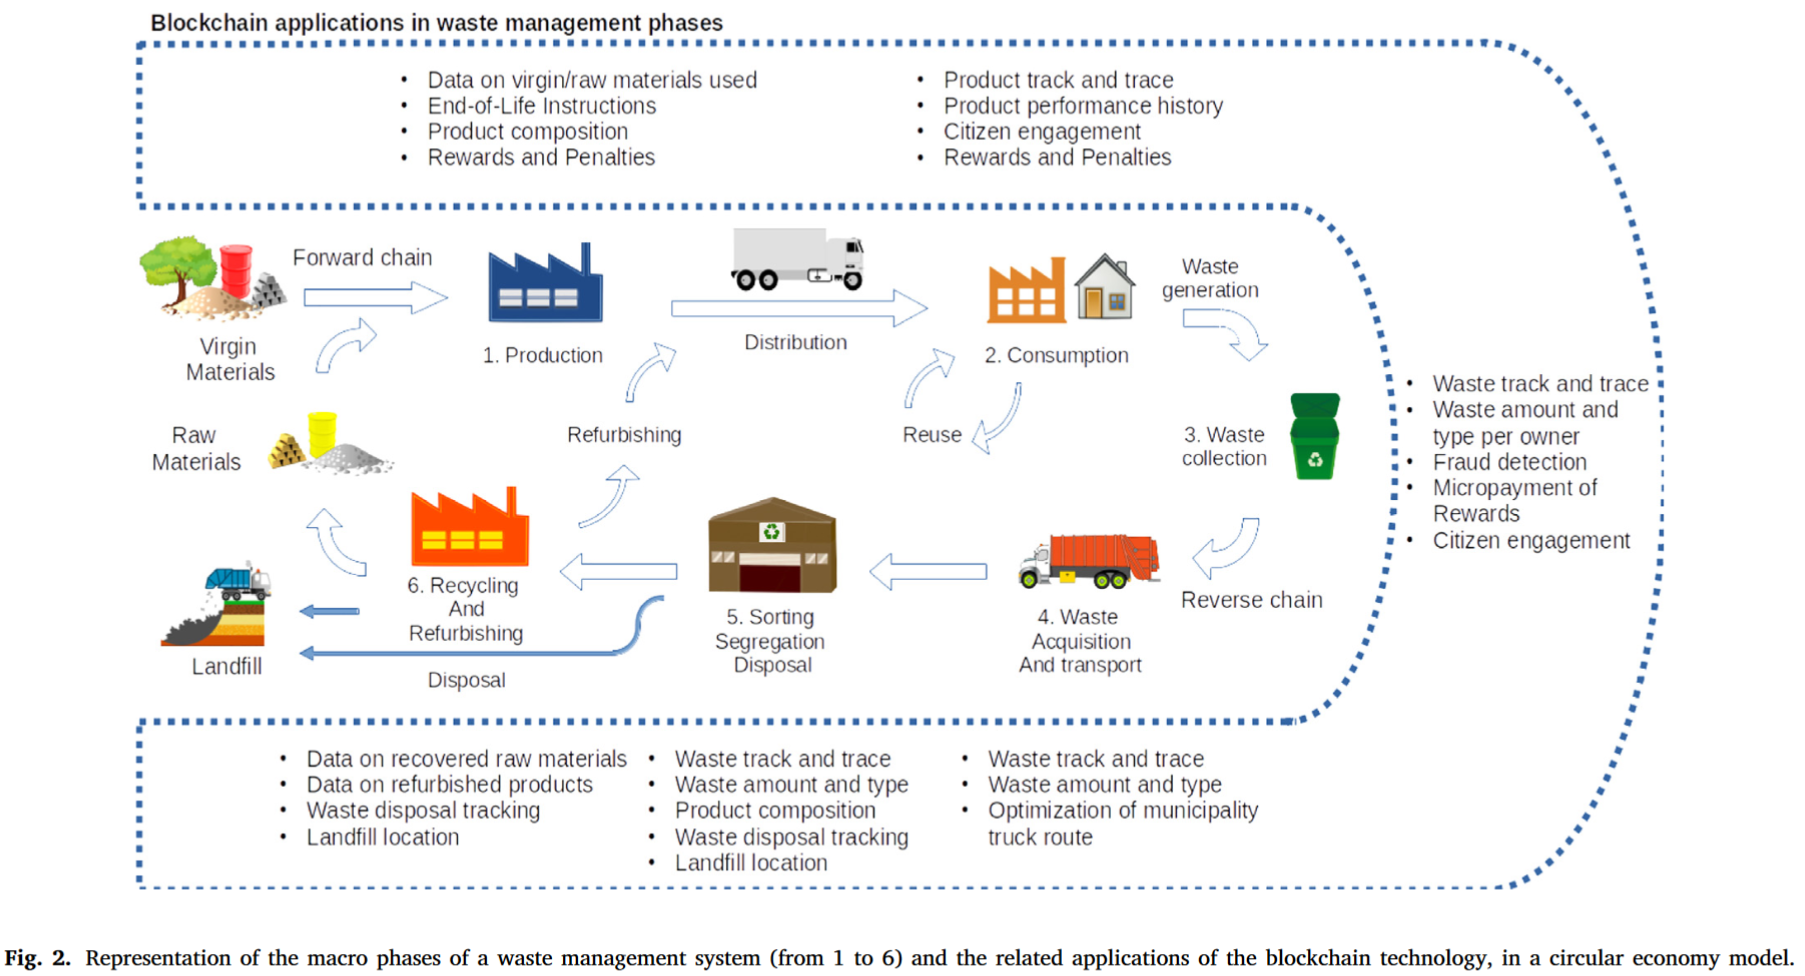
\includegraphics[width=1\textwidth]{./assets/baralla-model-1.png}
	\caption{Representación de las macro-fases de un sistema de gestión de residuos aplicando blockchain en un modelo de economía circular. Fuente: Baralla et al. (2023).}
	\label{fig:baralla-1}
\end{figure}

\begin{figure}[h]
	\centering
	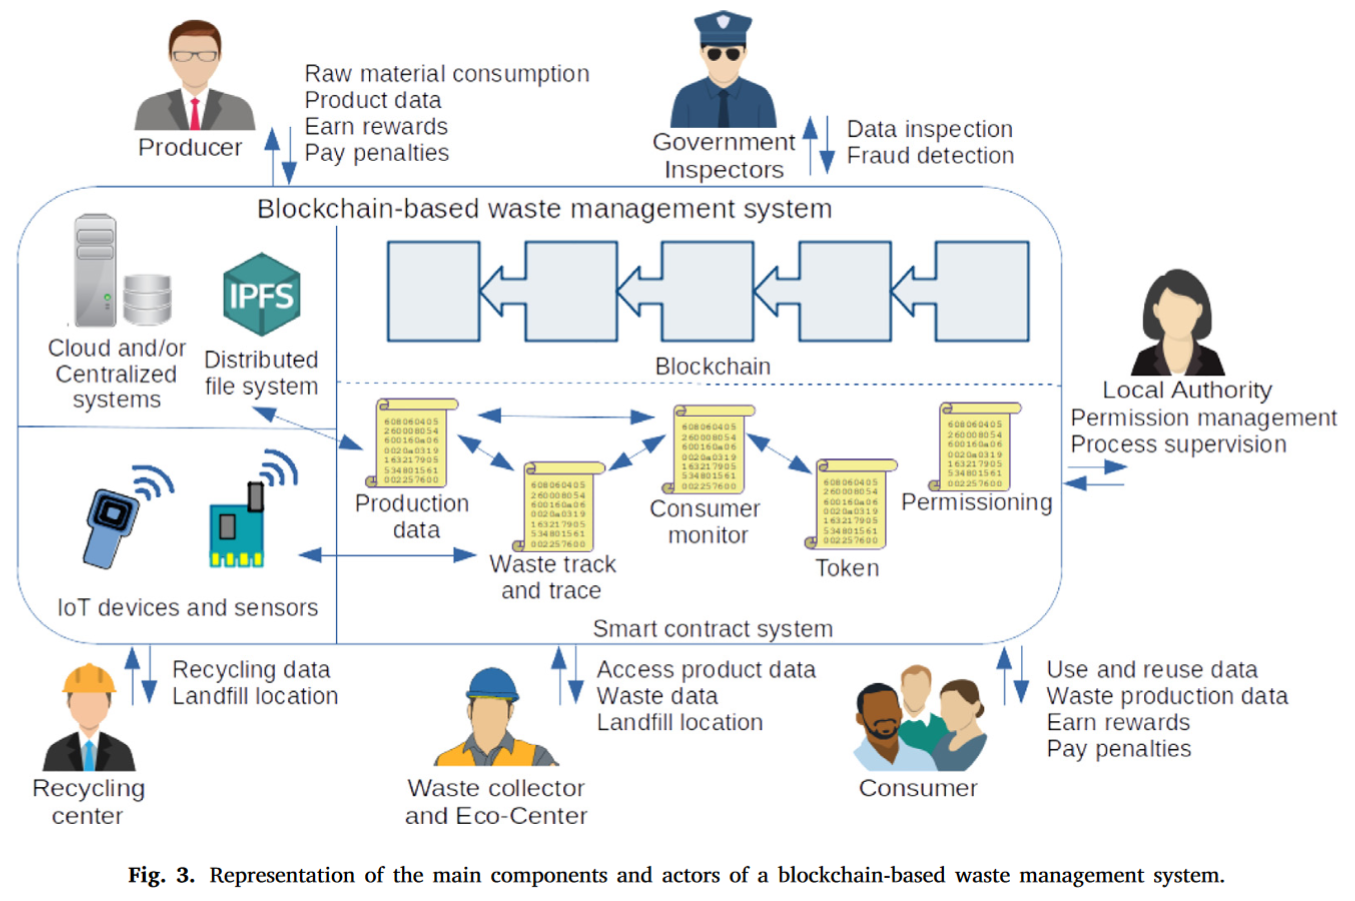
\includegraphics[width=1\textwidth]{./assets/baralla-model-2.png}
	\caption{Representación de los componentes principales y actores de un sistema de gestión de residuos basado en blockchain. Fuente: Baralla et al. (2023).}
	\label{fig:baralla-2}
\end{figure}

Las conclusiones destacan que la tecnología blockchain puede garantizar la transparencia, inmutabilidad, trazabilidad y permite compartir datos entre los actores del sistema, apoyando una gestión eficaz de los residuos. Además, puede fomentar la participación ciudadana a través de incentivos económicos con la emisión de criptomonedas por participar. Sin embargo, solo el 25\% de los estudios revisados proporcionan detalles técnicos sobre su sistema o su implementación, sugiriendo que el interés literario está apenas en sus comienzos. Además, la tecnología blockchain aún está en sus etapas iniciales, con algunos problemas críticos, particularmente para las blockchains públicas, incluyendo la escalabilidad, privacidad de datos, alto consumo de energía y bajo rendimiento.

\subsection{Modelo ZERO para el Reciclaje de Plásticos con Tecnología Blockchain}
El artículo "Investigating the Applicability of Blockchain Technology and Ontology in Plastics Recycling by the Adoption of ZERO Plastic Model" \cite{sandhiya2020investigating} explora cómo la tecnología blockchain puede revolucionar la industria del reciclaje de plásticos mediante la implementación de un modelo conocido como ZERO. Este modelo utiliza códigos QR, IoT y tecnología blockchain para crear un sistema de trazabilidad inmutable que asegura la transparencia y la responsabilidad a lo largo de todo el proceso de reciclaje.

\subsubsection{Descripción del Modelo}
El modelo ZERO se centra en superar los desafíos significativos de auditoría al desarrollar un sistema auditable, resistente al fraude y económicamente práctico. Este modelo rastrea los plásticos individuales desde el inicio hasta el final de su ciclo de vida, proporcionando una solución para mejorar la calidad y eficiencia del reciclaje.

Las principales decisiones de diseño en el modelo ZERO incluyen:
\begin{itemize}
    \item \textbf{Uso de Códigos QR:} Cada producto plástico producido se etiqueta con un código QR único que permite la trazabilidad del producto a lo largo de su ciclo de vida hasta su reciclaje.
    \item \textbf{Ontología:} La utilización de la ontología ayuda a reducir ambigüedades conceptuales y mejora la gestión de información en el ciclo de vida del producto.
    \item \textbf{Bines Inteligentes:} Los bines de reciclaje inteligentes aceptan solo plásticos con un código QR activo, garantizando que solo se reciclen materiales apropiados y no se contabilice múltiples veces el mismo residuo.
\end{itemize}

\subsubsection{Implementación Técnica}
La implementación técnica del modelo ZERO incluye varias innovaciones clave:
\begin{itemize}
    \item \textbf{QR Grabados Molecularmente:} Los códigos QR se insertan a nivel macromolecular en el polímero, lo que evita daños o manipulaciones y mantiene la integridad del código a lo largo del ciclo de vida del producto.
    \item \textbf{Uso de Blockchain:} La información del producto se registra en una blockchain durante su producción, creando un "gemelo digital" que permite rastrear el producto a lo largo de su vida útil.
    \item \textbf{Máquina con Lector de QR:} Las máquinas de reciclaje están equipadas con lectores de QR que verifican la validez del código antes de aceptar el plástico para reciclaje.
    \item \textbf{Pre-Clasificación Automática:} Gracias a la información del código QR, la máquina clasifica los plásticos según su huella de CO2 y otros parámetros, facilitando su procesamiento posterior.
\end{itemize}

\subsubsection{Incentivos}
El sistema de incentivos del modelo ZERO funciona de la siguiente manera:
\begin{itemize}
    \item \textbf{Recompensas Monetarias:} Los usuarios reciben recompensas monetarias por reciclar, lo que fomenta la participación activa en el proceso de reciclaje.
    \item \textbf{Recompensas para Recolectores:} Los recolectores de basura se benefician de nuevas fuentes de ingresos al entregar plásticos reciclables.
    \item \textbf{Incentivos para Cada Eslabón:} Cada participante en la cadena de reciclaje recibe una recompensa cuando el siguiente eslabón cumple su función, promoviendo así una cadena de incentivos que estimula el cumplimiento y la eficiencia.
\end{itemize}

Estas características del modelo ZERO demuestran un enfoque innovador y prometedor para abordar el problema del reciclaje de plásticos mediante el uso de tecnología avanzada, alineando los intereses económicos con los objetivos ambientales.

\subsubsection{Conclusiones}
El modelo ZERO presenta un enfoque integral en la gestión de reciclaje de plásticos, integrando tecnología de blockchain e Internet de las Cosas (IoT) para optimizar y transparentar el proceso. Las principales conclusiones y aspectos relevantes del modelo para este trabajo incluyen:

\begin{itemize}
    \item \textbf{Integración de IoT y Blockchain:} El uso combinado de códigos QR y contenedores inteligentes con tecnología blockchain permite rastrear y recompensar de manera eficiente la recolección de plásticos, garantizando la trazabilidad de cada artículo a lo largo de su ciclo de vida.
    \item \textbf{Recompensas Monetarias:} El sistema ofrece incentivos económicos directos a los usuarios por sus acciones de reciclaje, promoviendo una participación más activa en las prácticas de reciclaje sostenible.
    \item \textbf{Gemelos Digitales para el Rastreo:} Cada producto plástico se trackea individualmente mediante un "gemelo digital" utilizando códigos QR, lo que permite una gestión detallada y personalizada del reciclaje de cada ítem.
    \item \textbf{Beneficios para Recolectores de Basura:} El modelo proporciona nuevas fuentes de ingresos para los recolectores de basura, integrándolos como actores clave en el proceso de reciclaje sin perjudicar a los actores preexistentes del sistema.
    \item \textbf{Incentivos a lo Largo de la Cadena:} Se establece un sistema de recompensas en cascada, donde cada eslabón de la cadena recibe un incentivo cuando el siguiente cumple su función, fomentando la cooperación y el cumplimiento efectivo de cada fase del proceso.
\end{itemize}

\subsection{Uso de Blockchain y Marcadores Moleculares para el Manejo Sostenible de Residuos Plásticos}

El trabajo de Bhubalan et al. \cite{BHUBALAN2022113631} explora las aplicaciones del blockchain y los marcadores moleculares en el reciclaje de plásticos para promover una economía circular global. Los autores argumentan que el reciclaje es crucial para mantener bajo el consumo de energías renovables y optimizar la economía, al tiempo que se reduce la competencia por la biomasa.
A su vez destacan que a pesar del incremento en la conciencia pública sobre los impactos negativos de la contaminación por plásticos y la participación en programas de reciclaje, los sistemas actuales de gestión de desechos no procesan de manera efectiva los residuos plásticos para su reciclaje y reutilización.

Este artículo se centra en abordar las deficiencias en la gestión de residuos plásticos utilizando tecnología blockchain en combinación con el marcado molecular para rediseñar químicamente los plásticos, logrando así un reciclaje cerrado y manteniendo el valor de los plásticos sintéticos por un tiempo prolongado.

El artículo destaca que la tecnología blockchain facilita la trazabilidad del origen de los plásticos desde su producción hasta su disposición final de manera inmutable, transparente y segura. Además, apoya la economía circular mediante la transparencia de la información, la confiabilidad y la automatización, lo que permite aprovechar efectivamente las iniciativas de economía circular.

A su vez, analiza que el modelo económico circular de los plásticos enfrenta varios desafíos, como la necesidad de clasificar los plásticos basándose en el tipo de polímero y la trazabilidad del uso anterior. Una solución propuesta es el 'pasaporte digital del producto', que cierra la brecha de información al revelar datos verificables sobre el reúso, contenido y potencial de reciclaje del producto.

Los autores fundamentan que la aplicación de polímeros controlados por secuencia en blockchain es una tecnología clave para el reciclaje de plásticos, ya que proporciona un código único para la identificación auténtica y la trazabilidad de las transacciones de productos plásticos, minimizando así los residuos plásticos. 

\subsubsection{Conclusiones del Artículo}
\begin{itemize}
    \item El artículo destaca la importancia de identificar cada plástico individualmente para su reciclaje mediante tecnologías como el marcado molecular.
    \item Examina los altos costos asociados con la implementación de la tecnología blockchain, cuestionando su rentabilidad para plásticos de un solo uso.
    \item Discute cómo los marcadores moleculares podrían mejorar significativamente la trazabilidad y la autenticación de los plásticos reciclados.
    \item El estudio proporciona una visión integral de cómo la combinación de blockchain y tecnologías avanzadas de marcado puede revolucionar la gestión de residuos plásticos y avanzar hacia una economía circular a escala global.
\end{itemize}


\subsection{Aplicaciones de Blockchain en la Trazabilidad de la Cadena de Suministro para Sustentabilidad}

En la actualidad, existen aplicaciones productivas basadas en la tecnología blockchain que están demostrando que se pueden alcanzar mejores resultados en el reciclaje y proporcionar ventajas significativas tanto para productores como para consumidores. Estas aplicaciones abordan la trazabilidad desde el principio de la cadena de suministro, en lugar de comenzar el seguimiento al final de la vida útil del producto.

\subsubsection{Circularise}
Circularise es una plataforma líder en blockchain que ofrece pasaportes digitales de productos para la trazabilidad de extremo a extremo y el intercambio seguro de datos en cadenas de suministro industriales \cite{circularise2024}.

\textbf{Características destacadas de Circularise:}
\begin{itemize}
  \item \textbf{Transparencia en la Cadena de Suministro:} Circularise permite rastrear la sostenibilidad de los productos más allá del primer nivel de proveedores, usando pasaportes digitales que registran el origen del producto, la composición del material, y los datos ambientales, respaldados por la cadena de custodia impulsada por blockchain.
  \item \textbf{Recolección de Datos Primarios:} Facilita la recopilación de datos primarios a lo largo de la cadena de suministro para realizar evaluaciones completas del ciclo de vida (LCA) y calcular la huella de carbono del producto (PCF), estableciendo un registro confiable del impacto ambiental de un producto.
  \item \textbf{Cumplimiento Regulatorio:} Permite reportar contra indicadores clave de desempeño de sostenibilidad y agilizar los procesos de auditoría, compartiendo datos sobre el origen del producto, la huella de carbono, y cumpliendo con regulaciones y certificaciones como la regulación de baterías de la UE.
  \item \textbf{Privacidad de Datos:} Asegura la privacidad de los datos, permitiendo control total sobre qué datos compartir para cumplir con requisitos regulatorios y de clientes, mientras se mantiene información sensible protegida.
  \item \textbf{Integración con ERP:} Ofrece integración con sistemas ERP existentes a través de una API para automatizar el manejo de inventarios en masa y los pasaportes de productos digitales.
  \item \textbf{Apertura e Interoperabilidad:} Adopta un enfoque abierto e interoperable para eliminar silos de datos y conectar de manera fluida los datos a través de cadenas de suministro complejas.
  \item \textbf{Certificación ISCC Plus:} Circulor utiliza una blockchain pública descentralizada para garantizar que las empresas no puedan parecer más sostenibles de lo que son, utilizando la prueba de una afirmación de sostenibilidad a través de activos. Este principio es la base de la confianza en la integridad de los datos.
\end{itemize}

\subsubsection{Circulor}
Circulor es una plataforma de SaaS empresarial privada y basada en permisos, que ofrece soluciones avanzadas para la trazabilidad y la sostenibilidad en cadenas de suministro industriales. Utiliza tecnología de blockchain para proporcionar un seguimiento exhaustivo desde la fuente hasta el consumidor final, lo que permite a las empresas demostrar la procedencia responsable, mejorar su desempeño en ESG (Environmental, Social, and Governance), reducir las emisiones de gases de efecto invernadero y gestionar los riesgos asociados a la cadena de suministro \cite{circulor2024}

\textbf{Características destacadas de Circulor:}
\begin{itemize}
  \item \textbf{Plataforma Intuitiva:} La plataforma incluye interfaces de usuario intuitivas tanto en aplicaciones de escritorio para cargas manuales rápidas, como en aplicaciones móviles que facilitan la adopción del sistema por parte de los usuarios.
  \item \textbf{Integración y Interoperabilidad:} Diseñada para una fácil integración con plataformas empresariales existentes, permite una alimentación de datos sin interrupciones hacia el blockchain mediante APIs RESTful con protocolos de seguridad y autenticación.
  \item \textbf{Contribución a la Investigación y Normativas:} Apoya la interoperabilidad y ha contribuido a establecer las directrices de Blockchain del RMI, además de participar en investigaciones de vanguardia en el área.
  \item \textbf{Trazabilidad de Materiales y Productos:} Sus productos de trazabilidad rastrean el origen de materias primas y el flujo actual de materiales a través de los procesos de producción y transformaciones que sufren dentro de las cadenas de suministro de manufactura y reciclaje.
  \item \textbf{Sostenibilidad y Emisiones:} Circulor permite a los clientes medir dinámicamente sus emisiones atribuidas e inherentes en cada etapa de la cadena de suministro, mejorando los enfoques de evaluación del ciclo de vida actual.
  \item \textbf{Apoyo en ESG y Reciclaje en Circuito Cerrado:} La plataforma ayuda a definir los KPI de ESG basados en datos de trazabilidad, permitiendo a los clientes medir y comparar las credenciales de sostenibilidad de sus proveedores y alcanzar objetivos globales de ESG. Además, asegura el reciclaje en circuito cerrado de materiales como electrónicos, plásticos y baterías de vehículos eléctricos, demostrando que los procesos de reciclaje o disposición se llevan a cabo de manera responsable.
\end{itemize}

\subsubsection{Conclusiones}

\begin{itemize}
    \item La integración de tecnologías de trazabilidad desde la etapa de producción ha demostrado ser eficaz para generar mayor consciencia en cada eslabón de la cadena de suministro, contribuyendo así a incrementar las tasas de reciclaje de manera significativa.
    \item La capacidad de las empresas para certificar sus procesos como sostenibles se ve facilitada sin que esto implique un esfuerzo adicional considerable, permitiendo una validación eficiente de sus prácticas ambientales.
    \item Estas tecnologías no solo mejoran la sostenibilidad de los procesos mediante una gestión más eficiente de los recursos, sino que también optimizan la utilización de estos a lo largo de todo el ciclo de vida del producto.
    \item El uso de sistemas de trazabilidad robustos, como el blockchain, permite responsabilizar a los productores por su impacto ecológico, ofreciendo una herramienta transparente y fiable para medir y gestionar dicho impacto.
\end{itemize}

\end{document}
